
\documentclass{article}
\usepackage{graphicx}

\usepackage{listings}
\usepackage{color}
\usepackage{hyperref}
\hypersetup{colorlinks=True,citecolor=blue}

\definecolor{dkgreen}{rgb}{0,0.6,0}
\definecolor{gray}{rgb}{0.5,0.5,0.5}
\definecolor{mauve}{rgb}{0.58,0,0.82}

\lstset{frame=tb,
	language=Python,
	aboveskip=3mm,
	belowskip=3mm,
	showstringspaces=false,
	columns=flexible,
	basicstyle={\small\ttfamily},
	numbers=none,
	numberstyle=\tiny\color{gray},
	keywordstyle=\color{blue},
	commentstyle=\color{dkgreen},
	stringstyle=\color{mauve},
	breaklines=true,
	breakatwhitespace=true,
	tabsize=3
}

\begin{document}
	


%\renewcommand{\abstractname}{}    % clear the title
%\renewcommand{\absnamepos}{empty}

\title{RASSINE tutorial}

\author{Michael Cretignier\footnote{michael.cretignier@unige.ch} \\ University of Geneva}

\maketitle

\tableofcontents
\newpage
	
\section{Basic command}

This tutorial is to help you to use efficiently RASSINE. First check that you possess all the needed dependencies by running the test files Sect. \ref{individual} and Sect. \ref{timeseries}. Excepted pandas, all the libraries are quite common if you are a familiar python user.
	
You can familiarise with the code by reading, the \textbf{README.txt} file, the docstring on the parameters (\textbf{Docstring\_rassine.pdf}) as well as the main article.
	
\subsection{Individual spectra normalisation}
\label{individual}
	
 Open a terminal and move into the Rassine\_public directory containing the main codes and launch an Ipython session : 


\begin{lstlisting}
cd /Users/cretignier/Documents/GitHub/Rassine_public/
ipython 
run Rassine.py 
\end{lstlisting}

\begin{figure*}[h]
	\centering
	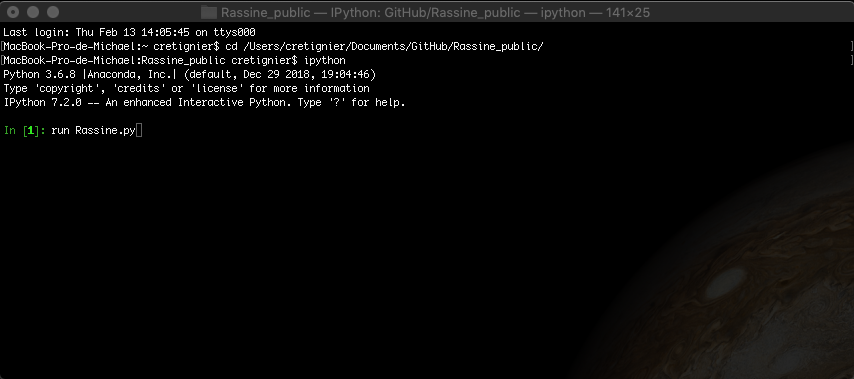
\includegraphics[width=12cm]{/Users/cretignier/Documents/LaTeX/Docstring/step1.png}
	\caption{Test the dependencies on your computer by running the Rassine.py code.}
	\label{FigInt6}
\end{figure*} 


If all the dependencies are installed the first graphical interface should appear. In this window the slider should work and your smoothed spectra should react in real time. Just follow the steps and communicate with the Sphinx in the terminal. If you managed to reach the end of the code, it means that you are now able to normalise spectra by changing the input spectrum file. But before that, let us rerun the test file without the Sphinx. To do so, you can just disable it by switching off the feedback button in the config file \textbf{Rassine\_config.py}. 
 \begin{lstlisting}
feedback = False        # run the code without graphical feedback and interactions with the sphinx (only wishable if lot of spectra)     
 \end{lstlisting}
 
 And in the previous terminal : 
 
 \begin{lstlisting}
 run Rassine.py 
 \end{lstlisting}
 
 By doing so, you are now configured in "complete automatic mode". You can basically measure the typical time to reduce one spectra in automatic mode depending on your computer performance. Keep in mind that this mode will not necessarily provide you the best result but is giving most of the time good first guess values for the parameter. The only parameters that are not automatic are the smoothing kernel and kernel length as well as the penalty law.
 
   \begin{lstlisting}
   par_smoothing_box = 6           # half-window of the box used to smooth (1 => no smoothing, 'auto' available)  <--- PARAMETER 2
   par_reg_nu = 'poly_1.0'    # penality-radius law          <--- PARAMETER 6
  \end{lstlisting}

Remark you can also switch on the smoothing in automatic mode by putting the 'auto' keyword, but usually the Savitchy-Golay filtering works in a quite large diversity of cases (excepted for SNR spectra lower than $\sim75$): 

   \begin{lstlisting}
par_smoothing_box = 'auto'           # half-window of the box used to smooth (1 => no smoothing, 'auto' available)  <--- PARAMETER 2
par_smoothing_kernel = 'erf' # 'rectangular','gaussian','savgol' if a value is specified in smoothig_kernel
\end{lstlisting}

\newpage
\subsection{Spectra time-series}
\label{timeseries}

RASSINE also offers an unique opportunity to normalise a spectra time-series (a series of spectra all coming from the same star). To do so, moves into the main directory, and launch the test file in an Ipython shell by running \textbf{Rassine\_trigger.py}.

\begin{lstlisting}
cd /Users/cretignier/Documents/GitHub/Rassine_public/
ipython 
run Rassine_trigger.py 
\end{lstlisting}

Hear that voice ? It is Victoria. She's there to warn you either when the Sphinx is waiting on your feedback or when a reduction step is finished. A problem with Victoria ? That's fine, you can select Daniel instead ! Bored by human voices ? You can also disable them in the \textbf{Rassine\_functions.py} file. 

\begin{lstlisting}
voice_name = ['Victoria', 'Daniel', None][0] #voice pitch of the auditive feedback
\end{lstlisting}

You can select the steps of the cascade that you want by switching on/off the buttons in the \textbf{Rassine\_trigger.py}. 

\begin{lstlisting}
preprocessed = 1
match_frame = 1
stacking = 1
rassine_normalisation_master = 1
rassine_normalisation = 1
rassine_intersect_continuum = 1
rassine_diff_continuum = 1
\end{lstlisting}

\newpage
\section{Spectra of different stars}

RASSINE can reduce spectra of different stars, but if so you will have to use the full automatic mode. First put all your spectra in a common directory and change the directory name of the \textbf{Rassine\_trigger.py} file as well as the instrument for the preprocessing in case of fits files. All your spectra should come from the same instrument. 

\begin{lstlisting}
instrument = 'HARPS'                                                     # instrument (either HARPS, HARPN, CORALIE or ESPRESSO for the moment)
dir_spec_timeseries = cwd+'/spectra_library/CenB/'   # directory containing the s1d spectra timeseries

\end{lstlisting}

Because all the spectra are now independent and do not share any information, you only have to preprocess them and to launch the Rassine normalisation in multiprocess:

\begin{lstlisting}
preprocessed = 1
match_frame = 0
stacking = 0
rassine_normalisation_master = 0
rassine_normalisation = 1
rassine_intersect_continuum = 0
rassine_diff_continuum = 0
\end{lstlisting}




\newpage
\section{Change the input spectrum of individual reduction}

You are now ready to normalise your own spectra (I am crossing the fingers for you). To do so, change the input spectrum name in the \textbf{Rassine\_config.py} file and switch on/off the feedback depending on your wish. 

\begin{lstlisting}
spectrum_name = cwd+'/spectra_library/spectrum_cenB.csv' # full path of your spectrum pickle/csv file
feedback = False        # run the code without graphical feedback and interactions with the sphinx (only wishable if lot of spectra)     
\end{lstlisting}

As a reminder, RASSINE was developed for 1d spectra, if you are trying to normalise a 2d spectrum, consider to switch on the feedbacks and keep an eye on the automatic value selected.

\section{Change the input spectra of time-series}

In a similar fashion that for individual spectra, change the input spectra directory in the \textbf{Rassine\_trigger.py} file. Indicate the instrument that will be used to preprocess your data in case of fits file and launch the \textbf{Rassine\_trigger.py } code.

\begin{lstlisting}

instrument = 'HARPS'                                                     # instrument (either HARPS, HARPN, CORALIE or ESPRESSO for the moment)
dir_spec_timeseries = cwd+'/spectra_library/CenB/'   # directory containing the s1d spectra timeseries
 
\end{lstlisting}




\end{document}
